%-----------------------------------
%
\chapter{Assembly}
%
%-----------------------------------

\AY{Different ways to put the above layers together/ordering them. Simulating RASPS and etc can go here?}


\section{Induction Heads}

\LS{Will write}

\section{Exchanging Heads for Layers}
We show that one can always exchange the computations performed by a transformer head with those of a transformer layer. 

\begin{enumerate}
    \item Both a head and a layer have their own separate parameters.
    \item Different heads compute different functions, which are then combined using the head combination function.
    \item A layer computes takes the previous layers' outputs as inputs and computes its own output.
\end{enumerate}

\section{\texorpdfstring{$n$}{n}-grams}
\AS{Will write}


\begin{figure}
    \centering

    \begin{tikzpicture}[
        tape node/.style={draw=ETHBlue!80,minimum size=0.85cm,fill=ETHBlue!20},
        head node/.style={draw=ETHGreen!80,circle,minimum size=0.65cm,fill=ETHGreen!60,text=white},
        attn arrow/.style={-{Latex[length=2.25mm,width=1.5mm]},ETHGreen!100},
        comb arrow/.style={-{Latex[length=2.25mm,width=1.5mm]},ETHRed!70},
        comb node/.style={draw=ETHRed!80,circle,minimum size=0.75cm,fill=ETHRed!40},
        ]

        % Draw tape
        \foreach \i/\y in {0/$\sym_1$,1/$\sym_2$,2/$\cdots$,3/$\sym_{\tstep-4}$,4/$\sym_{\tstep-3}$,5/$\sym_{\tstep-2}$,6/$\sym_{\tstep-1}$,7/$\symt$,8/$\cdots$} {
                \ifnum \i=7
                    \node[tape node,fill=ETHBlue!40] (tape-\i) at (0.85*\i,0) {\footnotesize \y};
                \else
                    \ifnum \i>3
                        \ifnum \i<7
                            \node[tape node,fill=ETHBlue!25] (tape-\i) at (0.85*\i,0) {\footnotesize \y};
                        \fi
                    \else
                        \node[tape node,fill=ETHBlue!15] (tape-\i) at (0.85*\i,0) {\footnotesize \y};
                    \fi
                    \ifnum \i>7
                        \node[tape node,fill=ETHBlue!15] (tape-\i) at (0.85*\i,0) {\footnotesize \y};
                    \fi
                \fi
            }

        % Draw attention heads
        \node[head node] (head-1) at (2,1.7) {\scriptsize \texttt{Head 3}};
        \node[head node] (head-2) at (3.5,1.7) {\scriptsize \texttt{Head 2}};
        \node[head node] (head-3) at (5,1.7) {\scriptsize \texttt{Head 1}};

        % Draw arrows from heads to tape
        \draw[attn arrow, ETHGreen!20] (head-1) to[out=270,in=90] (tape-0.north);
        \draw[attn arrow, ETHGreen!20] (head-1) to[out=270,in=90] (tape-1.north);
        \draw[attn arrow, ETHGreen!20] (head-1) to[out=270,in=90] (tape-3.north);
        % \draw[attn arrow, ETHGreen!20] (head-1) to[out=270,in=90] (tape-4.north);
        \draw[attn arrow, ETHGreen!20] (head-1) to[out=270,in=90] (tape-5.north);
        \draw[attn arrow, ETHGreen!20] (head-2) to[out=270,in=90] (tape-0.north);
        \draw[attn arrow, ETHGreen!20] (head-2) to[out=270,in=90] (tape-1.north);
        \draw[attn arrow, ETHGreen!20] (head-2) to[out=270,in=90] (tape-3.north);
        \draw[attn arrow, ETHGreen!20] (head-2) to[out=270,in=90] (tape-4.north);
        % \draw[attn arrow, ETHGreen!20] (head-2) to[out=270,in=90] (tape-5.north);
        \draw[attn arrow, ETHGreen!20] (head-3) to[out=270,in=90] (tape-0.north);
        \draw[attn arrow, ETHGreen!20] (head-3) to[out=270,in=90] (tape-1.north);
        \draw[attn arrow, ETHGreen!20] (head-3) to[out=270,in=90] (tape-3.north);
        \draw[attn arrow, ETHGreen!20] (head-3) to[out=270,in=90] (tape-4.north);
        \draw[attn arrow, ETHGreen!20] (head-3) to[out=270,in=90] (tape-5.north);
        \draw[attn arrow] (head-1) to[out=270,in=90] (tape-4.north);
        \draw[attn arrow] (head-2) to[out=270,in=90] (tape-5.north);
        \draw[attn arrow] (head-3) to[out=270,in=90] (tape-6.north);

        % Draw combiner node
        \node[comb node] (combiner) at (4.5,3.4) {$\headCombineFunc$};

        % Draw arrows from tape to combiner
        \draw[comb arrow] (head-1.north) to[out=90,in=270] (combiner.south);
        \draw[comb arrow] (head-2.north) to[out=90,in=270] (combiner.south);
        \draw[comb arrow] (head-3.north) to[out=90,in=270] (combiner.south);

        \node[fill=none] (out) at (0.5,4.25) {$\plm\left(\symt\mid\str_{<\tstep}\right)$};

        % Draw an arrow from the combiner to the output
        % \draw[comb arrow] (combiner.north) -- ++(0,1.25) node[above] {};
        % \draw (combiner) edge[comb arrow, right] node{\footnotesize $\outMtx$} (out.south);
        \draw[comb arrow] (combiner.north) to[out=90,in=270] (out.south) ;
        % \node[fill=none] (out) at (3.45,3.7) {\footnotesize $\outMtx$};
        \node[fill=none] (out) at (3.2,4.5) {\footnotesize $\softmax\left(\outMtx \; \cdot\right)$};

    \end{tikzpicture}
    \caption{A transformer LM can simulate a $4$-gram LM using \textcolor{ETHGreen}{3 heads}. The stronger arrows from the heads to the symbols show where the heads focus their attention.}
    \label{fig:transformer-n-gram-label}
    \vspace{-10pt}
\end{figure}


Ingredients:
\begin{enumerate}
    \item Hard attention (unique or averaging),
    \item Bounded or unbounded positional encodings,
    \item Logarithmic precision,
    \item One-hot symbol encodings, and
    \item $n - 1$ heads (or $n - 1$ layers).
\end{enumerate}

Given an $n$-gram LM $\plm$, we can construct an equivalent transformer LM $\plm'$ that looks back at the preceding $n - 1$ positions using $n - 1$ heads, each of them uniquely attending to exactly one position.
The symbols attended to can be used to identify the full history, which can be used to access the conditional distribution over the next symbol.

% We now outline the intuition behind the construction of a hard attention transformer LM simulating an \ngram LM, as first presented in \cref{fig:transformer-n-gram-label}.\footnote{For simplicity, we disregard the role of residual connections in the following outline. Residual connections are, however, considered in the full proof later.}
% To ease the exposition, we start with the final step of the construction: Assuming we have identified the appropriate history $\str^{\tstep - 1}_{\tstep - n + 1}$ after combining the head values using the head combining function $\headCombineFunc$, we show how $\tfpLM$ can encode the conditional probability distribution $\pLNSM\left(\sym_\tstep\mid\str_{\tstep- n + 1 : \tstep - 1}\right)$.
% The intuition of this step is simple: Knowing what the individual $\pLNSM\left(\sym_\tstep\mid\str^{\tstep - 1}_{\tstep - n + 1}\right)$ for $\sym_\tstep \in \eosalphabet$ are, we can simply put their logits into a vector and combine the constructed vectors for all possible histories into the output matrix $\outMtx$:\footnote{To be able to take the $\log$ of $0$ probabilities, we work over the set of \emph{extended} reals $\Rex = \R \cup \set{-\infty, \infty}$.}\textsuperscript{,}\footnote{Throughout the paper, we implicitly index the matrices directly with symbols and histories. We assume that the symbols and histories are ordered in some way and that the matrices are ordered accordingly.}
% \begin{equation}
%     \eOutMtx_{\sym, \str^{\tstep - 1}_{\tstep - n + 1}} \defeq \log{\pLNSM\left(\sym_\tstep\mid\str^{\tstep - 1}_{\tstep - n + 1}\right)}
% \end{equation}
% In the following, we write $\tfencfun\left(\str_{<\tstep}\right)$ as shorthand notation for $\tfencfun\left(\str_{<\tstep}\right) \defeq \fTransf\left(\vx_{\tstep - 1}^\tfnumlayer\right)$ (i.e., the representation which is linearly transformed by $\outMtx$ to compute $\pLM\left(\symt \mid \strlt\right)$ after normalization) where $\mX^\tfnumlayer = \tf\left(\staticRepr\right)\left(\strlt\right)$.
% If we one-hot encode the identified history with $\tf$ as
% \begin{equation}
%     \tfencfun\left(\str_{<\tstep}\right) \defeq \onehot{\str^{\tstep - 1}_{\tstep - n + 1}}
% \end{equation}
% we can then, using the formulation of the transformer LM from \cref{def:transformer-plnsm}, use the $\tfencfun\left(\str_{<\tstep}\right)$ to look up the appropriate column in $\outMtx$ containing the logits of the conditional probabilities given the identified history for all possible $\sym_\tstep \in \eosalphabet$, i.e., $\left(\outMtx \ \tfencfun\left(\str_{<\tstep}\right)\right)_\sym = \log\pLNSM\left(\sym \mid\str^{\tstep - 1}_{\tstep - n + 1}\right)$.

% We now consider the preceding step of the simulation: Identifying the history given that the $n - 1$ heads identified the symbols $\sym_1, \ldots, \sym_{n - 1}$ in the positions they attended to.
% If we concatenate the values of the $n - 1$ heads into a vector $\vv$, this vector of size $\left(n - 1\right)|\eosalphabet|$ will contain the \defn{multi-hot} representation of the history of interest:
% \begin{equation}
%     \vv = \begin{pmatrix}
%         \onehot{\sym_1} \\
%         \vdots          \\
%         \onehot{\sym_{n - 1}}
%     \end{pmatrix}
% \end{equation}
% and $\vv_{\idxi |\eosalphabet| + \idxj} = 1$ if and only if $\symordering\left(\sym_\idxi\right) = \idxj$ for a bijection $\symordering\colon \eosalphabet \to \NTo{|\eosalphabet|}$ that determines the indices of the one-hot representations of the symbols.
% We would then like to transform this vector into a vector $\vu \in \R^{|\alphabet|^{n - 1}}$ such that
% \begin{equation}
%     \evu_{\idxi} = 1 \iff \idxi = \anOrdering\left(\sym_1, \ldots, \sym_{n - 1}\right)
% \end{equation}
% for a bijection $\anOrdering\colon \underbrace{\eosalphabet \times \cdots \times \eosalphabet}_{n - 1\text{ times}} \to \NTo{|\eosalphabet|^{n - 1}}$.
% This can be equivalently written as
% \begin{equation}
%     \evu_{\idxi} = 1 \iff \evv_{\idxj |\eosalphabet| + \symordering\left(\sym_\idxj\right)} = 1 \text{ for all } \idxj = 1, \ldots, n - 1
% \end{equation}
% where $\idxi = \anOrdering\left(\sym_1, \ldots, \sym_{n - 1}\right)$.
% This is an instance of performing the logical \texttt{AND} operation, which can be implemented by an MLP as described in \cref{fact:and}.
% This MLP will form the transformation $\headCombineFunc$ combining the information obtained from all the heads of the transformer.

% This brings us to the final part of the proof: Identifying the symbols at the previous $n - 1$ positions by the $n - 1$ transformer heads.
% To show how this can be done, let us consider the parameters we can still set to define a transformer:
% \begin{itemize}[itemsep=0.5pt,parsep=0.5pt]
%     \item The position-augmented symbol representations $\posInEmbedding$.
%           Inspired by concurrent work from \citet{merrill2023expressive}, we use the representations of the form
%           \begin{equation}
%               \posInEmbeddingFun{\symt, \tstep} = \begin{pmatrix}
%                   \onehot{\symt} \\
%                   \sqrt{\frac{1}{\tstep}} \\
%                   \sqrt{1 - \frac{1}{\tstep}} \\
%                   \sqrt{\frac{1}{\tstep + 1}} \\
%                   \sqrt{1 - \frac{1}{\tstep + 1}} \\
%                   \vdots \\
%                   \sqrt{\frac{1}{\tstep + n - 1}} \\
%                   \sqrt{1 - \frac{1}{\tstep + n - 1}}
%               \end{pmatrix} \in \R^{2 n}
%           \end{equation}
%           This results in vectors $\posInEmbedding\left(\sym_\tstep, \tstep\right)$ of size $|\eosalphabet| + 2 + 2 \left(n - 1\right)$.
%           Note that such a symbol representation function can be implemented by concatenating or adding symbol- ($\onehot{\symt}$) and position- ($\sqrt{\frac{1}{\tstep}}, \ldots, \sqrt{1 - \frac{1}{\tstep + n - 1}}$) specific components, which is in line with most practical implementations of the transformer architecture.
%     \item The attention scoring function $\tfscorefun$.
%           We will use the standard dot-product scoring function
%           \begin{equation} \label{eq:transformer-ngram-function}
%               \tfscorefun\left(\vq, \vk\right) \defeq \innerProd{\vq}{\vk}.
%           \end{equation}
%           $\tfscorefun$ will, together with the positional encodings, allow us to easily single out the relevant positions in the string.
%     \item The parameters of each of the attention heads, that is, the transformations $\qTransf$, $\kTransf$, and $\vTransf$.
%           Each of those will take the form of a linear transformation of the symbol (and positional) representations.
%           We describe them and their roles in more detail below.
% \end{itemize}
% The parameters of all the heads will be identical, with the only difference being a single parameter that depends on the ``index'' of the head, $h$.
% In the following, we describe the construction of a single head.
% At any time step $\tstep$ (i.e., when modeling the conditional distribution $\pLNSM\left(\sym_\tstep \mid \str_{<\tstep}\right)$), the head $h$ will attend to the symbol at position $\tstep - h$, $\sym_{\tstep - h}$.
% In \cref{fig:transformer-n-gram-label}, for example, \texttt{Head $3$} attends to the position $\tstep - 3$, which is denoted by the stronger arrow to that position.
% We now describe the individual transformations $\qTransf_h$, $\kTransf_h$, $\vTransf_h$, and $\oTransf_h$ of the head $h$.
% All of them will be \emph{affine} transformations.
% Since we are considering only the first layer of the transformer, we can think of the inputs to the layer as the original symbol representations together with their position encodings (rather than some contextual representations at higher levels).
% As mentioned, the head $h$ will be responsible for identifying the symbol at position $\tstep - h$.
% Therefore, we want it to put all its attention to this position.
% In other words, given the query $\vq_{\tstep - 1}$, we want the attention function in \cref{eq:transformer-ngram-function} to be uniquely maximized by the key of the symbol at position $\tstep - h$.
% Notice that, therefore, the key does not have to depend on the identity of the symbol at position $\tstep - h$---only the positional information matters.
% Let us then consider the following query and key transformations for head $h$:\looseness=-1
% \begin{align}
%     \qTransf_h\colon & \posInEmbedding\left(\sym_\tstep, \tstep\right) \mapsto \begin{pmatrix}
%       \sqrt{\frac{1}{\tstep}} \\
%       \sqrt{1 - \frac{1}{\tstep}}
%     \end{pmatrix} \\
%     \kTransf_h\colon & \posInEmbedding\left(\sym_\tstep, \tstep\right) \mapsto \begin{pmatrix}
%       \sqrt{\frac{1}{\tstep + h}} \\
%       \sqrt{1 - \frac{1}{\tstep + h}}
%     \end{pmatrix}.
% \end{align}
% Given such a query and such keys, the scoring function computes
% \begin{equation} \label{eq:hard-attention-scores}
%     \tfscorefun\left(\vq_\tstep, \vk_\idxj\right) = \innerProd{\begin{pmatrix}
%       \sqrt{\frac{1}{\tstep}} \\
%       \sqrt{1 - \frac{1}{\tstep}}
%     \end{pmatrix}}{\begin{pmatrix}
%       \sqrt{\frac{1}{\idxj + h}} \\
%       \sqrt{1 - \frac{1}{\idxj + h}}
%     \end{pmatrix}}.
% \end{equation}
% \cref{eq:hard-attention-scores} is an inner product between two unit vectors, and is therefore maximized if and only if they are the same, that is, if $\idxj = \tstep - h$. This is exactly the position that we want the head $h$ to attend to.\footnote{Note that while the choice of the positional encodings in this construction is uncommon in practice, the popular sinusoidal positional encodings \citep{Vaswani2017} have also been linked to the ability of the transformer-based models to attend to specific positions of interest based on linear transformations of the positional encodings \citep{Vaswani2017}.}
% % This means that the hard attention we use will put all its probability mass to exactly the position we intended it to.
% Intuitively, both transformations keep only the positional information.
% The query transformation ``injects'' the knowledge of which position should maximize the attention score, while the key transformation simply ``exposes'' the positional information about the symbol.
% The constants $1$ and $-1$ and the index of the position ensure that the inner product simply computes the difference between the position of the symbol and the position of interest.

% This leaves us with the question of how to use the position of the symbol of interest ($\tstep - h$) to extract the one-hot encoding of the symbol at that position.
% Due to the information contained in the symbol representations $\posInEmbedding\left(\sym_\idxj\right)$, this is trivial:
% \begin{equation} \label{eq:hard-attention-values}
%     \vTransf\colon \posInEmbedding\left(\sym_\tstep, \tstep\right) \mapsto \onehot{\sym_\idxj}.
% \end{equation}
% With this, the identity of the symbol is carried forward through the attention mechanism.
% Notice that the only head-depend transformation is the query transformation---it depends on the index of the head, determining the position of interest, meaning that every head defines a different query transformation, while the keys and values transformations are the same among all heads.
% This concludes the outline of the proof.




\section{Computing MOD without positional encodings}

\WM{Will write}

\section{Dyck Language}

\AX{Will write}\CW{Will also write}

\section{ELIZA}

\DF{Will write}

\section{Comparison}
\label{sec:assembly_comparison}

\AY{Comparing numerical values. The part that makes this slightly unstraightforward is ensuring that the result is in the desired Boolean representation}

Assumptions:
\begin{itemize}
    \item Function from $\Z\times\Z\to \left\{\begin{bmatrix}
            -1\\\phantom- 1
        \end{bmatrix}, \begin{bmatrix}
            \phantom- 1\\-1
        \end{bmatrix}\right\}$
\end{itemize}

This requires access to $\pm\frac{1}{i+1}$ in some dimensions $2k_0-1,2k_0$.

    First we explain how to simulate a comparison of two count terms $C_1(i)\leq C_2(i)$. Then, we describe how to extend this to %simulate, for sets of indices $X_1$ and $X_2$, the expression \[\sum_{x\in X_1} c_{x} \cdot C_x(i) \leq \sum_{x\in X_2} c_{x} \cdot C_x(i).\]
    compare linear combinations of count terms.

    Suppose that we want to compare $C_1$ and $C_2$ in dimensions $2k_1-1,2k_1$ and $2k_2-1,2k_2$, and put the result in dimension $2k_3-1,2k_3$. Initially, the residual stream looks like this:
    \begin{equation*}
    \begin{blockarray}{cccc}
        & & i & \\
        \begin{block}{c[ccc]}
                &  & \vdots &  \\
               2k_0-1 & \cdots & -\frac{1}{i+1} & \cdots \\[6pt]
                2k_0 & \cdots & +\frac{1}{i+1} & \cdots \\
                & & \vdots & \\[6pt]
               2k_1-1 & \cdots & -\frac{C_1(i)}{i+1} & \cdots \\[6pt]
                2k_1 & \cdots & +\frac{C_1(i)}{i+1} & \cdots \\
                & & \vdots & \\
               2k_2-1 & \cdots & -\frac{C_2(i)}{i+1} & \cdots \\[6pt]
                2k_2 & \cdots & +\frac{C_2(i)}{i+1} & \cdots \\
              & & \vdots & \\
               2k_3-1 & \cdots & 0 & \cdots \\[6pt]
                2k_3 & \cdots & 0 & \cdots \\
                & & \vdots & \\
        \end{block}
    \end{blockarray}
    \end{equation*}

    \newcommand{\clipfn}{\operatorname{gtz}}

    We construct a feed-forward layer that computes the function:
    \[\clipfn(X(i)) = \min\left(\frac{0.5}{i+1},\frac{X(i)}{i+1}-\frac{0.5}{i+1}\right)-\min\left(0,\frac{X(i)}{i+1}\right).
    \qquad
    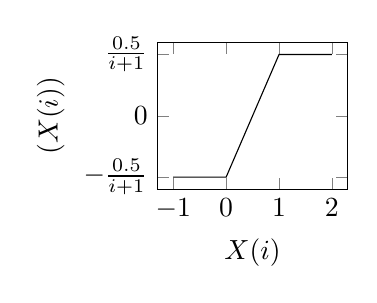
\begin{tikzpicture}[baseline=0.8cm]
    \begin{axis}[width=4cm,xlabel={$X(i)$},xtick={-1,0,1,2},ylabel={$\clipfn(X(i))$},ytick={-0.5,0,0.5},yticklabels={$-\frac{0.5}{i+1}$,$0$,$\frac{0.5}{i+1}$}]
    \addplot[mark=none,samples at={-1,0,1,2}] { min(0.5, x-0.5)-min(0,x) };
    \end{axis}
    \end{tikzpicture}\]

    Observe that $\clipfn(C_2(i)-C_1(i)+0.5)$ equals $\frac{0.5}{i+1}$ if $C_1(i)\leq C_2(i)$, and $-\frac{0.5}{i+1}$ otherwise.
    This is because the counts $C_1(i),C_2(i)$ must be integers, so if $C_1(i)\leq C_2(i)$, then $C_2(i)-C_1(i)+0.5\geq 0.5$, and the expression will evaluate to $\frac{0.5}{i+1}$. Otherwise, $C_2(i)-C_1(i)+0.5<-0.5$, and the expression will evaluate to $-\frac{0.5}{i+1}$.

    It is straightforward, then, to use the construction for $\min$/$\max$ from above to produce a feed-forward layer that computes $\clipfn\left(C_2(i)-C_1(i)\right)$. Essentially, we use $W_1$ to compute the values (using the pre-existing values from the residual stream)

    \[\frac{0.5}{i+1}, \frac{C_2(i)-C_1(i)+0.5}{i+1}, -\frac{C_2(i)-C_1(i)+0.5}{i+1}\]

    Then we use $W_2$ to compute

    \[\frac{0.5}{i+1}+\ReLU\left(\frac{0.5}{i+1}-\frac{C_2(i)-C_1(i)+0.5}{i+1}\right)-\ReLU\left(\frac{0.5}{i+1}-\frac{C_2(i)-C_1(i)-0.5}{i+1}\right)\]
    which equals $\clipfn(C_2(i)-C_1(i))$ as desired.

    Similarly, it is straightforward to construct a feed-forward layer to compare linear combinations of count terms. That is, for disjoint sets of indices $K_1$ and $K_2$, to compute
    \[\clipfn\left(\sum_{k\in K_2} c_{k} \cdot C_k(i) -\sum_{k\in K_1} c_{k} \cdot C_k(i)\right).\]

    So we can construct a feed-forward layer $f:\R^d\to\R^d$ that computes in each dimension $i$ the following

    \[f\left(\begin{bmatrix}
        v_1\\
        v_2\\
        \vdots\\
        v_{2k_3-1}\\
        v_{2k_3}\\
        \vdots\\
        v_{d-1}\\
        v_{d}\\
    \end{bmatrix}\right) =\begin{bmatrix}
        \clipfn(v_1)\\
        \clipfn(v_2)\\
        \vdots\\
        \clipfn\left(\sum_{k\in K_2} c_{k} \cdot C_k(i) -\sum_{k\in K_1} c_{k} \cdot C_k(i)\right)\\
        \clipfn\left(\sum_{k\in K_2} c_{k} \cdot C_k(i) -\sum_{k\in K_1} c_{k} \cdot C_k(i)\right)\\
        \vdots\\
        \clipfn(v_{d-1})\\
        \clipfn(v_{d})\\
    \end{bmatrix}. \]

    This truncates all positive values in the residual stream at this point to be $\frac{0.5}{i+1}$ at position~$i$, and all nonpositive values to be $-\frac{0.5}{i+1}$. As a result, the next application of LayerNorm (with appropriate parameter settings) scales every single value to $\pm 1$. In particular, all previously-computed Boolean values are preserved, and the newly-computed dimensions $2k_3-1,2k$ hold the correct Boolean value based on the desired comparison